\باب{اینٹینا اور شعاعی اخراج}

\حصہ{تعارف}

\حصہ{تاخیری دباو}
کسی بھی اخراج شعاع کے نظام میں موج کے ترسیل کے لئے درکار دورانیہ اہمیت رکھتا ہے۔یوں شکل \حوالہ{شکل_اینٹینا_تاخیری_رو} میں دکھائے تار میں برقی رو سے پیدا میدان کا اثر نقطہ نقطہ \عددیء{N} پر کچھ وقفے سے ہو گا۔خالی خلاء میں یہ وقفہ موج کو تار سے نقطے تک پہنچنے کا دورانیہ \عددیء{\frac{r}{c}} ہے جہاں
 \عددیء{c=\SI{3e8}{\meter/\second}} خالی خلاء میں  شعاع کی رفتار ہے۔یوں نقطہ \عددیء{N} کے نقطہ نظر سے تار میں برقی رو
\begin{align}
I=I_0 \cos \omega t
\end{align} 
کی بجائے
\begin{align}\label{مساوات_اینٹینا_تاخیری_رو}
[I]=I_0 \cos \omega  \left (t-\frac{r}{c} \right)
\end{align} 
لکھی جا سکتی ہے جہاں \عددیء{[I]} \اصطلاح{تاخیری برقی رو}\فرہنگ{تاخیری!برقی رو}\حاشیہب{retarded current}\فرہنگ{retarded!current} کہلاتی ہے۔تاخیری تفاعل کو چکور قوصین میں بند لکھا جاتا ہے۔تاخیری برقی رو لکھتے ہوئے وقت \عددیء{t} کی جگہ تاخیری وقت \عددیء{(t-\tfrac{r}{c})} استعمال کیا جاتا ہے۔

\begin{figure}
\centering
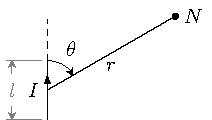
\includegraphics{figAntennaRetardedCurrent}
\caption{برقی رو گزارتی تار کی چھوٹی لمبائی}
\label{شکل_اینٹینا_تاخیری_رو}
\end{figure}

مساوات \حوالہ{مساوات_اینٹینا_تاخیری_رو} کہتا ہے کہ نقطہ \عددیء{N} پر لمحہ \عددیء{t}  پر پیدا اثر،  گزرے  لمحے \عددیء{(t-\tfrac{r}{c})} پر تار میں برقی رو کا اثر ہے جہاں تار سے \عددیء{N} تک فاصلہ \عددیء{r} ہے۔تار سے \عددیء{N} تک شعاع پہنچنے کا دورانیہ \عددیء{\tfrac{r}{c}} ہے۔

گزشتہ بابوں میں تاخیری اصطلاح کا ذکر کئے بغیر ہم تاخیری تفاعل استعمال کرتے رہے ہیں۔امواج کی بات کرتے ہوئے \عددیء{\cos (\omega t -\beta x)} استعمال کیا گیا جس میں \عددیء{\tfrac{\omega}{\beta}=c} کے استعمال سے
\begin{align}
\cos (\omega t -\beta x)=\cos \omega\left( t- \frac{x}{c}\right)
\end{align}
لکھا جا سکتا ہے  جو تاخیری تفاعل کو ظاہر کرتی ہے۔

مساوات \حوالہ{مساوات_اینٹینا_تاخیری_رو} کی دوری سمتیہ شکل
\begin{align}
[I]=I_0 e^{j \omega (t-r/c)}=I_0 e^{j(\omega t-\beta r)}
\end{align}
ہے۔اسی طرح کثافت برقی رو کی تاخیری دوری سمتیہ شکل
\begin{align}
[\kvec{J}]=\kvec{J}_0 e^{j(\omega  t -\beta r)}
\end{align}
ہو گی جسے استعمال کرتے ہوئے تاخیری مقناطیسی دباو
\begin{align}
[\kvec{A}]=\int_h \frac{\mu [\kvec{J}]}{4\pi r} \dif h
\end{align}
لکھا جائے گا۔اسی طرح تاخیری حجمی کثافت چارج
\begin{align}
[\rho_h]=e^{-r} \cos \left[\omega \left(t-\frac{r}{c} \right) \right]
\end{align}
لکھتے ہوئے تاخیری برقی دباو
\begin{align}
[V]=\int_h \frac{[\rho_h]}{4\pi \epsilon r} \dif h
\end{align}
لکھا جائے گا۔ باب-\حوالہ{باب_میکس_ویل} کے آخر میں مساوات \حوالہ{مساوات_میکس_ویل_تاخیری_سمتی_دباو} اور مساوات \حوالہ{مساوات_میکس_ویل_تاخیری_غیر_سمتی_دباو} کے بائیں ہاتھ کے تفاعل کو چکور قوصین میں لکھ کر موج کی رفتار \عددیء{c} لیتے ہوئے اور فاصلے  کو کروی محدد کے رداس \عددیء{r} سے ظاہر کرنے سے  یہی مساوات حاصل ہوتے ہیں۔


\حصہ{مختصر جفت قطبی اینٹینا}
مختصر لمبائی کے سیدھے موصل تار کو عموماً مختصر \اصطلاح{ جفت قطب}\فرہنگ{جفت قطب!مختصر}\حاشیہب{short dipole}\فرہنگ{dipole!short} کہا جاتا ہے۔مندرجہ ذیل گفتگو میں مختصر جفت قطب کی لمبائی محدود ہو گی۔لامحدود حد تک کم لمبائی کی صورت میں اسے صغاری جفت قطب\فرہنگ{صغاری جفت قطب}\حاشیہب{infinitesimal} کہا جائے گا۔

خطی نوعیت کے کسی بھی اینٹینا کو متعدد تعداد کے سلسلہ وار جڑے مختصر جفت قطبوں کا مجموعہ تصور کیا جا سکتا ہے لہٰذا مختصر جفت قطب کی خاصیت جانتے ہوئے زیادہ لمبے جفت قطب یا مختلف انداز میں جڑے موصل  تاروں کی خاصیت جاننے میں مدد ملے گی۔ 

آئیں شکل \حوالہ{شکل_اینٹینا_جفت_قطب}-الف میں دکھائے مختصر جفت قطب پر غور کریں جس کی لمبائی \عددیء{l} طول موج سے بہت کم \عددیء{l\ll \lambda} ہے۔جفت قطب کے سروں پر موصل چادر بطور  کپیسٹر  بوجھ کردار ادا کرتے ہیں۔جفت قطب کی مختصر لمبائی اور اس کے سروں پر موصل چادر مل کر جفت قطب  کی پوری لمبائی پر تقریباً برابر برقی رو رکھنے میں مدد دیتے ہیں۔جیسے شکل-الف میں دکھایا گیا ہے، جفت قطب کو متوازن ترسیلی تار سے طاقت مہیا کی جا سکتی ہے۔یہ فرض کرتے ہوئے کہ ترسیلی تار سے شعاعی اخراج نہیں ہوتی، اس کے موجودگی کو نظر انداز کیا جائے گا۔جفت قطب کے سروں پر نسب موصل چادروں کے شعاعی اخراج کو بھی نظر انداز کیا جائے گا۔جفت قطب کی موٹائی \عددیء{d} اس کے لمبائی سے بہت کم \عددیء{d\ll \lambda} ہے۔ان حقائق کو مد نظر رکھتے ہوئے تحلیلی تجزیے کی خاطر جفت قطب کو شکل \حوالہ{شکل_اینٹینا_جفت_قطب}-ب کی طرح تصور کیا جا سکتا ہے۔ایسا جفت قطب یکساں برقی رو \عددیء{I} گزارتا، \عددیء{l} لمبائی کا تار معلوم ہو گا جس کے دونوں سروں پر برابر مگر الٹ قطب کے چارج \عددیء{\mp q} ہوں جہاں چارج \عددیء{q} اور برقی رو \عددیء{I} کا تعلق
\begin{align}
I=\frac{\partial q}{\partial t}
\end{align}
ہے۔ 

آئیں لامحدود وسعت کی خالی خلاء میں جفت قطب کے میدان حاصل کریں۔جفت قطب کے وسط کو کروی محدد کے مرکز اور لمبائی کو \عددیء{z} محدد پر رکھتے ہوئے آگے بڑھتے ہیں۔کسی بھی نقطہ \عددیء{N} پر عموماً آپس میں عمودی تین میدان \عددیء{E_r}، \عددیء{E_{\theta}} اور \عددیء{E{\phi}} پائے جائیں گے۔

\begin{figure}
\centering
\begin{subfigure}{0.4\textwidth}
\centering
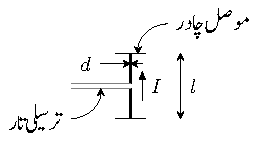
\includegraphics{figAntennaShortDipole}
\caption*{الف: متوازن ترسیلی تار سے جفت قطب کو طاقت مہیا کی گئی ہے۔}
\end{subfigure}%
%
\begin{subfigure}{0.4\textwidth}
\centering
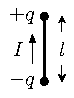
\includegraphics{figAntennaShortDipoleAsShortWire}
\caption*{ب: جفت قطب بطور چھوٹی تار}
\end{subfigure}%
\caption{جفت قطب}
\label{شکل_اینٹینا_جفت_قطب}
\end{figure}
